% !TeX program = lualatex
% !TeX encoding = utf8
% !TeX spellcheck = uk_UA
% !BIB program = biber
% !TeX root =../LabWork.tex

%\addbibresource{LabWork1.bib}
\expandafter\graphicspath\expandafter{\expandafter{\currfilebase/pic}}
\usetikzlibrary{arrows.meta}
\tikzset{
every info/.style={font=\small},
}

\abstract{Експериментально визначити горизонтальну і вертикальну складові, а також магнітне нахилення місцевого геомагнітного поля.}

\keywords{Магнітне поле Землі, горизонтальна складова, вертикальна складова, метод імплікації.}

\apparatus{Котушки Гельмгольца, магнітна стрілка зі шкалою, тесламетр з датчиком Хола для вимірювання величини магнітного поля.}
%===============================================================================%

\chapter{Вимірювання магнітного поля Землі}
\makeworktitle

\section*{Рекомендована література }
\begin{enumerate}
	\item \fullcite{Siv3}\\[0.5ex]
	      Рекомендується прочитати: \emph{\S\S~49 -- 53, 55, 56}.
	\item \fullcite{Mat3}\\[0.5ex]
	      Рекомендується прочитати: \emph{Глава 6, зокрема варто приділити увагу \S~39}.
\end{enumerate}


\section{Теоретичне підґрунтя}

\subsection{Земний магнетизм}

Про існування магнетизму було відомо з глибокої давнини. Вважається, що перший компас з'явився в Китаї. У 1600 році в книзі  <<Про магніті, магнітних тілах і про великий магніт~--- Землю>> У.~Гільбертом  було дано уявлення про причини земного магнетизму. У 1785 почалися розробки способу вимірювання напруженості магнітного поля, що базується на методі крутного моменту, запропонованому Ш. Кулоном. У 1839 К. Гаусс теоретично обґрунтував метод вимірювання горизонтальної складової вектора магнітного поля планети. На початку XX ст. було визначено зв'язок між магнітним полем Землі і її будовою.

Однак, факт існування цього загадкового фізичного явища природи для сучасної науки як і раніше багато в чому неясний. Вже з середини XX століття загальноприйнято, що походження геомагнітного поля і основні чинники його еволюції пов'язані з процесами в рідкому зовнішньому ядрі Землі. Причина подібної впевненості полягає в наступному. Сукупність спостережних даних про магнітне поле Землі переконує нас в тому, що воно має планетарний характер і його джерела повинні знаходитися глибоко під поверхнею Землі.

Спроба пов'язати таке магнітне поле з величезним постійним магнітом входить в протиріччя з помітним зростанням температури вглиб Землі. Справді, феромагнітні властивості зникають при досягненні критичної температури, яка називається \emph{точкою Кюрі}, та й сам образ гігантського постійного магніту десь в глибині Землі не виглядає реалістичним.

Ще одним джерелом магнітного поля Землі в принципі міг би служити розподіл зарядів, в результаті якого область між земною поверхнею і іоносферою являє собою гігантський конденсатор. Обертання Землі призводить до руху заряду цього конденсатора і електричний струм, який виникає таким чином, створює магнітне поле. Однак оцінки показують, що його напруженість набагато нижча ніж та, що спостерігається.

Ще одна з причин походження магнітного поля Землі може бути пов'язана з явищем електромагнітної індукції Фарадея. Цей механізм генерації магнітного поля називається \emph{механізмом динамо}. Вперше механізм динамо був запропонований на початку XX століття  Дж. Лармором для пояснення походження магнітного поля Сонця. Пізніше з дією цього механізму стали пов'язувати походження магнітних полів майже всіх небесних тіл, що мають магнітне поле. Суть механізму динамо зазвичай пояснюють як створення магнітного поля завдяки руху електропровідної рідини (плазми). Однак, пояснити походження геомагнітного поля механізмом динамо теж непросто. Справа в відомому правилі Ленца, згідно з яким додатковий струм, який з'являється в рамці зі струмом, що рухається в початковому (затравочному) магнітному полі, напрямлений таким чином, щоб зменшити затравочне магнітне поле. Іншими словами, обертання потоків провідної рідини не може призводити до самозбудження магнітного поля.

Вказати конкретний реалістичний механізм, який призводить до підсилення затравочного магнітного поля в результаті дії електромагнітної індукції, вдалося лише в 50-60 рр. XX ст. Ганнесом Альвеном. Суть ідеї полягає в тому, що магнітне поле у вакуумі, яке створюється електричним струмом, перпендикулярно до цього струму. Однак виявилося, що магнітне поле в хаотичному, турбулентному або конвективному потоці, усереднене по пульсаціям цього потоку, набуває компоненти, паралельної до електричного струму. Якщо спочатку у нас заряджена рідина, що диференціально обертається (різні частини повертаються навколо загальної осі обертання з різною кутовою швидкістю) створює <<звичайне>> магнітне поле перпендикулярне до струму, то згодом рідина буде захоплювати магнітне поле і витягувати його вздовж напряму свого руху, утворюючи тороїдальні силові лінії. Цей механізм створення тороїдального поля відомий як омега-ефект.

\subsection{Виміри}

Основні виміри %будуть
побудовані на принципі \textbf{імплікації постійного поля}, величина і напрям якого відомі, на невідоме магнітне поле Землі. Горизонтальна компонента магнітного поля Землі
$ {}^{h}\vec{B}_{E} $ %формула для левых индексов, другие варианты здесь:     https://tex.stackexchange.com/questions/11542/left-and-right-subscript-superscript
розраховується із напряму результуючої магнітної індукції ${}^{h}\vec{B}_{R}$:
%
\begin{equation} \label{Horizontalcomponent} %%%% нужно сбросить номер уравнения, вроде через \setcounter, хз
    \vec{B}_{R} =  \vec{B}_{H} +  \vec{B}_{E}
\end{equation}


Індикатором напряму результуючої \textbf{магнітної індукції} виступить магнітна стрілка з лімбом. Стрілку потрібно встановити за напрямом горизонтальної компоненти $ {}^{h}\vec{B}_{E} $ магнітного поля Землі.

%Припустимо, що ми змогли забезпечити
Нехай забезпечено
додаткове однорідне поле $ {}^{h}\vec{B}_{H} $.
Стрілка відхилиться на кут $\alpha$ і показуватиме напрям горизонтальної компоненти результуючого поля ${}^{h}\vec{B}_{R}$ (рис.~\ref{vectordiagram}).


%На рис.~\ref{vectordiagram} зображені горизонтальні компоненти поля в загальному випадку.
%%Компоненти, які зображено штриховими лінями, мають місце у випадку зміни полярності додаткового поля (зміни напряму струму).
\begin{figure}[ht!] \centering
%%\subfloat[ \label{picture1} ]{
%%    \includegraphics[width=0.5\textwidth]{images/vectordiagram.png}
%%    }
\subfloat[Горизонтальна площина\label{horizontal} ]{
    \begin{tikzpicture}
    \draw[->, ultra thick, arrows={-latex}]
    (0,0) coordinate (O)
    -- (3,-1) coordinate (be) node[below left] {
      ${}^{h}\vec{B}_{E}$};

    \draw[->, ultra thick, arrows={-latex}]
    (O) -- (3,2) coordinate (br) node[above] {
               ${}^{h}\vec{B}_{R}$ }
    pic[pic text=$\alpha$, draw=orange, <->, angle eccentricity=1.2, angle radius=1cm, arrows={-latex}]
    {angle=be--O--br};

    \draw[->, ultra thick, arrows={-latex}]
    (O)  -- (0,3) coordinate (bh) node[left] {
        ${}^{h}\vec{B}_{H}$  };

    \draw[gray] (be) -- (br) -- (bh);

    \draw[gray, dashed, ->, arrows={-latex}]
    (O) -- (0,-3) coordinate (d);

    \draw[gray, dashed] (be) -- (3,-4) coordinate (dn) -- (d);

    \draw[gray, dashed, ->, arrows={-latex}] (O) -- (dn);

    \draw[red, dashed] (-0.9,0.3) node[above left] { \color{red} \textbf{S}} -- (O);
    \draw[blue, dashed] (be) -- (3.9,-1.3) node[right] {\color{blue} \textbf{N}};

    \draw
     pic[pic text=$\varphi$, draw=black, angle eccentricity=1.5, angle radius=0.6cm, pic text options={above left}]
    {angle=be--O--bh};

    \draw[->, arrows={-latex}]
    pic[pic text=$\beta$, draw=black, <->, angle eccentricity=1.2, angle radius=1.5cm, arrows={-latex}]
    {angle=br--O--bh};

    \end{tikzpicture}
      }
\hspace{0.08\linewidth}
\subfloat[Вертикальна площина\label{vertical}]{
    \begin{tikzpicture}

    \draw[->, ultra thick, arrows={-latex}]
    (O) -- (3,0) coordinate (beh) node[above] {
      $ {}^{h}\vec{B}_{E} $};

    \draw[->, ultra thick, arrows={-latex}]
    (O) -- (0,-3.5) coordinate (bev) node[below] {
      $ {}^{v}\vec{B}_{E} $};

    \draw[gray, dashed, ->, arrows={-latex}]
    (O) -- (3,-3.5) coordinate (bea);

    \draw[gray, dashed]
    (beh) -- (bea) -- (bev);

    \draw[->, arrows={-latex}]
    pic[pic text=$\theta$, draw=black, <-, angle eccentricity=1.2, angle radius=1.5cm, arrows={-latex}]
    {angle=bea--O--beh};

    \draw[red, dashed] (-1,0) node[left] { \color{red} \textbf{S}} -- (O);
    \draw[blue, dashed] (beh) -- (4,0) node[right] {\color{blue} \textbf{N}};
    \end{tikzpicture}
      }
    \caption{Векторна діаграма складових магнітного поля у   горизонтальній~(\subref{horizontal}) та  вертикальній~(\subref{vertical}) площинах. Компоненти, зображені штриховими лініями, відповідають випадку зміни полярності додаткового поля $ {}^{h}\vec{B}_{H} $ (зміни напряму струму).}
    \label{vectordiagram}
\end{figure}

З \textbf{теореми синусів} маємо:
\begin{equation} \label{SinTheorem}
    \frac{\sin{\alpha}}{\sin{\beta}} =
    \frac{\sin{\alpha}}{\sin (\varphi - \alpha)} =
    \frac{  {}^{h}\vec{B}_{H}
           }{
           {}^{h}\vec{B}_{E}
           }
\end{equation}

Для спрощення розрахунків %і оцінок похибок
розглядається
%В особливому випадку
випадок, коли вісь котушок перпендикулярна до напряму ``Північ -- Південь'' ($\varphi = 90^{\circ}$):
%; застосовується співвідношення:
%
\begin{equation} \label{specialcase}
   {}^{h}\vec{B}_{E} =  {}^{h}\vec{B}_{H} \cdot \ctg{\alpha}
\end{equation}

%що значно спрощує розрахунки і оцінки похибок.

Поле  $ {}^{h}\vec{B}_{H} $ пропорційно силі струму $I_{H}$: %, яка вимірюється безпосередньо.
%Коефіціент пропорційності залежить від конфігурації котушки , що створює поле, і називається калібровочним коефіціентом. Отже, маємо:
%
\begin{equation} \label{B_h}
     {}^{h}\vec{B}_{H} = C \cdot I_{H},
\end{equation}
де $C$ --- калібровочний коефіціент; залежить від конфігурації котушки.

Тоді з рівнянь \eqref{SinTheorem}, \eqref{B_h} %ми отримаємо:
маємо:
%%
\begin{equation} \label{h_B_E}
     {}^{h}\vec{B}_{E} \cdot  \frac{\sin{\alpha}}{\sin{\beta}} = C \cdot I_{H}.
\end{equation}

В експерименті визначається залежність $\frac{\sin{\alpha}}{\sin{\beta}}$ від $C \cdot I_{H} $, --- вона має бути лінійною.
З нахилу графіка цієї залежності безпосередньо визначається
%
величина, обернена
%зворотня
до горизонтальної складової магнітного поля Землі
%($1/\prescript{h}{}{{B_{E}}}$),
$({}^{h}\vec{B}_{E})^{-1}$:
%визначається безпосередньо з нахила графіка цієї залежності, вона має бути лінійною.
%
\begin{equation} \label{fsin}
        \frac{\sin{\alpha}}{\sin{\beta}} = \frac{1}{{}^{h}\vec{B}_{E}} \cdot C \cdot I_{H}.
\end{equation}

Якщо стрілку з лімбом встановити в вертикальній площині, можна безпосередньо заміряти кут $\theta$ (рис.~\ref{vertical}), з якого розрахувати вертикальну компоненту магнітного поля Землі ${}^{h}\vec{B}_{E}$ та сумарну індукцію $B_{E}$:
%%
\begin{align}\label{VerticalComp.MagneticFieldEarth}
    {}^{v}\vec{B}_{E} &=   {}^{h}\vec{B}_{E} \cdot \tg{\theta}, \\
     B_{E} &= \sqrt{ {}^{h}\vec{B}_{E}^2 + {}^{v}\vec{B}_{E}^2 }
\end{align}

\section{Експериментальне устаткування}
%\subsection{Будова установки}
Схема експериментальної установки зображена на рисунку \ref{Exp.equip}.

Котушки Гельмгольца з'єднані послідовно і підключені до джерела постійного струму через реостат та амперметр.

\begin{figure}[!h] \centering
%\subfloat[ \label{picture2} ]{
%    \includegraphics[width=0.5\textwidth]{images/Experimental equipment.png}
%    }

%\subfloat[ \label{picture1} ]{
     \begin{tikzpicture}
        \draw (5.5,0) node[below] {1} -- (0,0)
              to[battery] (0,4) --++(1,0)
              to[ampermeter] ++ (2,0)
              to[resistor] ++ (1,0) --++ (6,0)
              to ++(0,-4) -- (8,0) node[below] {1};
        \draw[thick, teal] (8.76,1.27) [partial ellipse=-90:220:1cm and 2cm];
        \draw[thick, teal] (6.26,1.27) [partial ellipse=-90:220:1cm and 2cm];
        \draw (6.26,-0.73) node[below] {2} -- (8.76,-0.73) node[below] {2};

        \draw[ultra thick, blue!50] (7.51,1.27) ellipse (0.75 and 0.25);
        \draw[ultra thick, blue!50, ->, -latex] (7.2,1.17) -- (8.02,1.37);

        \draw[red] (1,-1) -- (3,-1) --
              (3,1.8) -- (5,1.8) to[resistor, fill=red] ++ (1,0)  -- (8,1.8);
        \draw[red, very thick] (0,-2) rectangle (2.5,-0.5);
        \draw[red] (0.8,-1.2) -- (1.8,-1.8) -- (3,-1.8);

        \node[blue!50, text width=2cm] at (11.5,1.27) {Магнітна стрілка}; \draw[blue!50] (10.5,1.27) -- (8.5,1.27);

        \node[teal] at (7.5,-1.8) {Котушки Гельмгольца};

        \node[red, text width=3cm] at %(1.5,0.5)
        (-2,-0.7)
        {Тесламетр};

        \node[red] at (3.5,2.5) {Датчик Холла};

        \node[orange, text width=3cm] at (-2,2) {Джерело постійного струму};

    \end{tikzpicture}
 %   }

    \caption{Схема експериментальної установки: котушки Гельмгольца, джерело постійного струму, реостат, амперметр  з'єднані послідовно. Для вимірювання магнітного поля -- теслометр з датчиком Холла. Для вимірювання компонент магнітного поля Землі -- магнітометр з магнітною стрілкою та лімбом (на схемі -- магнітна стрілка).  }
    \label{Exp.equip}
\end{figure}

Магнітне поле вимірюється теслометром з датчиком Холла, який фіксує компоненту магнітної індукції, що паралельна осі датчика.

Важливо, щоб його напрям співпадав з напрямком осей котушок.
Щуп датчика встановлюється точно всередині пристрою Гельмгольца.

Чутливості теслометра не вистачає для вимірювання полей з індукцією порядка поля Землі.
Тому прилад застосовується для визначення калібровочного коефіцієнту $C$, який отримують з графіка залежності горизонтальної компоненти магнітної індукції $ {}^{h}\vec{B}_{H}$ від струму $I_{H}$ котушок \eqref{B_h}.

%\subsection{}

Для вимірювання горизонтальної компоненти магнітного поля Землі  $ {}^{h}\vec{B}_{E}$
використовується магнітометр з магнітною стрілкою, який має лімб з поділами, і може
встановлюватись уздовж проекції лінії індукції результуючого магнітного поля $\vec{B}_{R}$ на площину обертання
%, в якій обертається стрілка.
стрілки.

В роботі вивчають залежність кута $\alpha$ від індукції поля котушок $ {}^{h}\vec{B}_{H}$
за малих струмів, де $\alpha$  -- кут відхилення магнітної стрілки від її положення рівноваги.

Індукцію поля котушок  $ {}^{h}\vec{B}_{H} $ визначають з сили струму $I_{H}$ через котушки за допомогою калібровочного коефіціенту $K$.



\section{Хід роботи}

\subsection{Залежність  $ {}^{h}\vec{B}_{H} $ від $I_{H}$}

Встановлюємо датчик Холла всередині пристрою Гельмгольца, точно по центру.
\textit{До початку вимірювань %теслометр необхідно встановити на нуль. Ми
знімаємо покази теслометра, які слугуватимуть нульовим рівнем для наших даних.}

Знімаємо залежність горизонтальної компоненти магнітної індукції $ {}^{h}\vec{B}_{H} $ від струму  $I_{H}$ котушок. Діапазон зміни струму -- від 0 до 2 А.

\subsection{Залежність  $\alpha$ від $I_{H}$}

Замість датчика Холла за допомогою штативу встановлюємо магнітометр з магнітною стрічкою так, щоб центр лімбу знаходився точно в центрі пристрою Гельмгольца, а сам лімб був розташований точно в горизонтальній площині.

Визначаємо напрямок ``Північ--Південь'' на кільці з поділками за відсутності струму у котушках (рис.~\ref{compasH}). Для більш докладного визначення напряму стрілку треба легко відхилити від положення рівноваги кілька разів. \textit{Можлива сила тертя (що досить мала) може бути зменшена легким постукуванням по штативу.}

Проводимо вимірювання кута відхилення магнітної стрілки від положення рівноваги (напрямку ``Північ--Південь'' цієї стрілки) як функції малих струмів у котушці.
%
Повторюємо серію вимірювань після зміни напрямку струму в котушці на протилежний.

\textit{При вимірюванні точного кута повинні бути зафіксовані показання обох кінців стрілки.}

\begin{figure}
    \centering

\subfloat[Горизонтальна площина \label{compasH}]{
    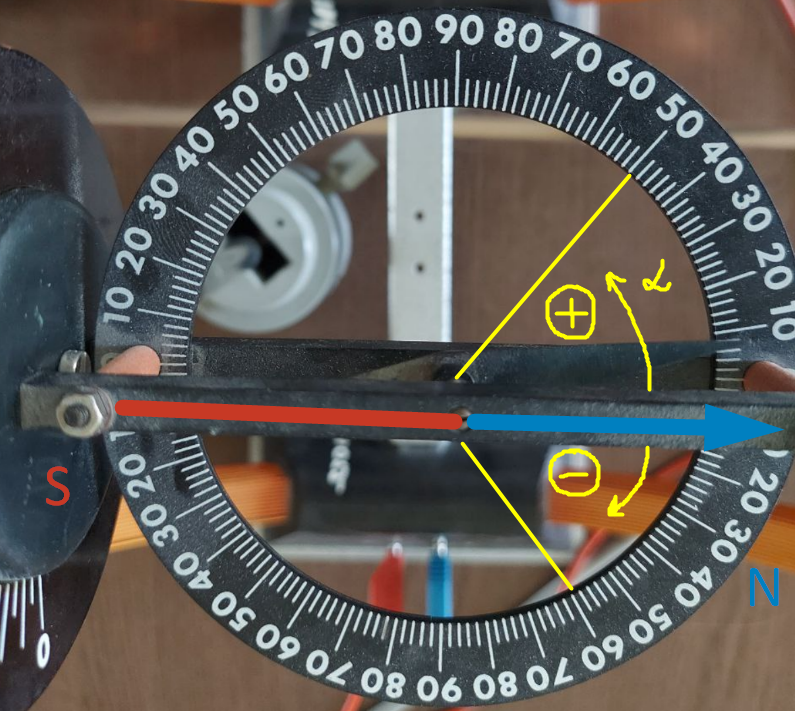
\includegraphics[height=0.39\linewidth]{compas.png}
    }
\subfloat[Вертикальна площина \label{compasV}]{
    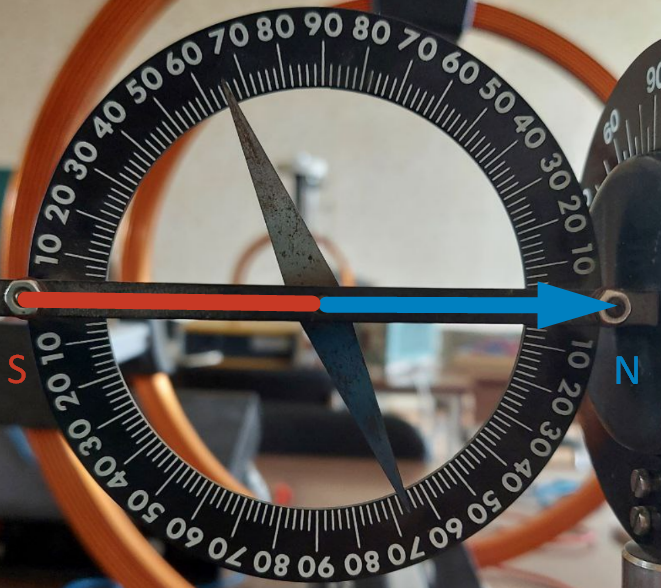
\includegraphics[height=0.39\linewidth]{compasV.png}
    }

    \caption{Магнітометр та напрямок ``Північ--Південь''}
    \label{compas}
\end{figure}

\subsection{Виміри  $\theta$}

За відсутності струму котушок лімб магнітометра повертаємо у вертикальну площину так, щоб магнітна стрілка вказувала кут нахилу. %Необхідно
Вісь обертання має співпадати з напрямком ``Північ--Південь'' (рис.~\ref{compasV}). З метою перевірки магнітометр повертаємо на $180^{\circ}$ і повторюємо виміри.


\section{Завдання}


\section{Контрольні запитання}



\section{Розрахункові завдання}


\end{document}
